\chapter{Test} \label{cap4}
In questo capitolo finale vengono presentati alcuni test effettuati nelle varie fasi dell'approccio precedentemente elencate. Come primo test vediamo la bontà dei vari classificatori-poselet. Successivamente vengono mostrati alcuni test di esecuzione.

\section{Classificatori Poselet}
Sono stati addestrati 7 tipi di classificatori-poselet: per ognuno di essi abbiamo da 1 a 3 classificatori: i classificatori di ogni tipo avranno gli stessi keypoints ma possono disporsi in modo differente nello spazio. Vediamo in dettaglio il loro numero e il tipo di poselet classificato

\begin{itemize}
\item 3 classificatori per la poselet contenente i keypoints: Occhio Sinistro/Destro, Naso, Orecchio Sinistro %face1
\item 2 classificatori per la poselet contenente i keypoints: Occhio Sinistro/Destro, Naso, Orecchio Sinistro/Destro %face12
\item 3 classificatori per la poselet contenente i keypoints: Occhio Sinistro/Destro, Naso, Orecchio Destro %face13
\item 3 classificatori per la poselet contenente i keypoints: Occhio Sinistro/Destro, Naso, Orecchio Sinistro/Destro, Spalla Sinistra/Destra, Gomito Sinistro/Destro %frontal2
\item 3 classificatori per la poselet contenente i keypoints: Occhio Sinistro/Destro, Naso, Orecchio Sinistro/Destro, Spalla Sinistra/Destra, Fianchi Sinistro/Destro %frontal22
\end{itemize}

Come è facilmente deducibile leggendo i keypoints presenti nei vari classificatori, essi individuano la parte superiore del corpo, soprattutto la zona relativa la faccia. Con questi classificatori quindi siamo abbastanza in grado di rilevare la parte superiore di persone poste in modo frontali a noi.\\
Per ogni classificatore poselet, riportiamo in basso la loro matrice di confusione e una poselet-patch presa dal training set: il classificatore è stato applicato a 300 campioni positivi e 800 campioni negativi. Tutti questi campioni non sono stati utilizzati nella fase di training. 

\begin{figure}[h]
 \centering
 \subfloat {\includegraphics[width=3cm]{cap4/ace1_11}} 
 \hspace{5mm}
 \subfloat {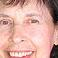
\includegraphics[width=3cm]{cap4/face1_2}}
 \hspace{5mm}
 \subfloat {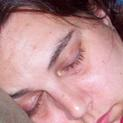
\includegraphics[width=3cm]{cap4/face1_3}}
 \vspace{5mm}
 
  \resizebox{.2\textwidth}{!}{%
 \begin{tabular}{|c | c|}
 \hline
 271 & 30 \\ \hline
 3 & 497 \\ 
 \hline
\end{tabular}%
}
\hspace{5mm}
\resizebox{.2\textwidth}{!}{%
\begin{tabular}[scale=1.5]{|c | c|}
 \hline
 265 & 36 \\ \hline
 14 & 486 \\ 
 \hline
\end{tabular}%
}
\hspace{5mm}
\resizebox{.2\textwidth}{!}{%
\begin{tabular}[scale=1.5]{|c | c|}
 \hline
 259 & 42 \\ \hline
 22 & 478 \\ 
 \hline
\end{tabular}%
}
\caption{Matrici di confusione per i classificatori-poselets tipo 1}
\label{table-deepnet}
 \end{figure}


\begin{figure}[h]
 \centering
 
 \subfloat {
\includegraphics[width=3cm]{cap4/face12_1}} 
 \hspace{5mm}
 \subfloat {
\includegraphics[width=3cm]{cap4/face12_2}}
 \vspace{5mm}
 
\resizebox{.2\textwidth}{!}{%
\begin{tabular}[scale=1.5]{|c | c|}
 \hline
 271 & 30 \\ \hline
 0 & 500\\ 
 \hline
\end{tabular}%
}
\hspace{5mm}
\resizebox{.2\textwidth}{!}{%
\begin{tabular}[scale=1.5]{|c | c|}
 \hline
 271 & 30 \\ \hline
 8 & 492 \\ 
 \hline
\end{tabular}%
}
\caption{Matrici di confusione per i classificator-poselets tipo 2}
\label{table-deepnet}
 \end{figure}



\begin{figure}[h]
 \centering
 \subfloat {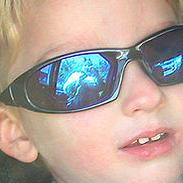
\includegraphics[width=3cm]{cap4/face13_1}} 
 \hspace{5mm}
 \subfloat {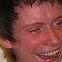
\includegraphics[width=3cm]{cap4/face13_2}}
 \hspace{5mm}
 \subfloat {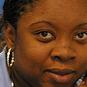
\includegraphics[width=3cm]{cap4/face13_3}}
 \vspace{5mm}
 
  \resizebox{.2\textwidth}{!}{%
 \begin{tabular}{|c | c|}
 \hline
 266 & 35 \\ \hline
 8 & 492 \\ 
 \hline
\end{tabular}%
}
\hspace{5mm}
\resizebox{.2\textwidth}{!}{%
\begin{tabular}[scale=1.5]{|c | c|}
 \hline
 253 & 48 \\ \hline
 31 & 469 \\ 
 \hline
\end{tabular}%
}
\hspace{5mm}
\resizebox{.2\textwidth}{!}{%
\begin{tabular}[scale=1.5]{|c | c|}
 \hline
 276 & 25 \\ \hline
 44 & 456 \\ 
 \hline
\end{tabular}%
}
\caption{Matrici di confusione per i classificatori-poselets tipo 3}
\label{table-deepnet}
 \end{figure}


\begin{figure}[h]
 \centering
 \subfloat {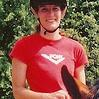
\includegraphics[width=3cm]{cap4/frontal2_1}} 
 \hspace{5mm}
 \subfloat {
\includegraphics[width=3cm]{cap4/frontal2_2}}
 \hspace{5mm}
 \subfloat {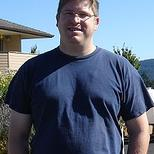
\includegraphics[width=3cm]{cap4/frontal2_3}}
 \vspace{5mm}
 
  \resizebox{.2\textwidth}{!}{%
 \begin{tabular}{|c | c|}
 \hline
 223 & 78 \\ \hline
 61 & 439 \\ 
 \hline
\end{tabular}%
}
\hspace{5mm}
\resizebox{.2\textwidth}{!}{%
\begin{tabular}[scale=1.5]{|c | c|}
 \hline
 22 & 279 \\ \hline
 0 & 500 \\ 
 \hline
\end{tabular}%
}
\hspace{5mm}
\resizebox{.2\textwidth}{!}{%
\begin{tabular}[scale=1.5]{|c | c|}
 \hline
 227 & 74 \\ \hline
 70 & 430 \\ 
 \hline
\end{tabular}%
}
\caption{Matrici di confusione per i classificatori-poselets tipo 4}
\label{table-deepnet}
 \end{figure}
 
 
 
 \begin{figure}[h!b]
 \centering
 \subfloat {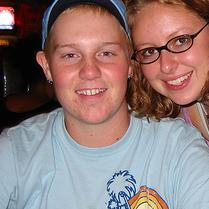
\includegraphics[width=3cm]{cap4/frontal22_1}} 
 \hspace{5mm}
 \subfloat {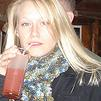
\includegraphics[width=3cm]{cap4/frontal22_2}}
 \hspace{5mm}
 \subfloat {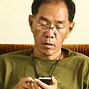
\includegraphics[width=3cm]{cap4/frontal22_3}}
 \vspace{5mm}
 
  \resizebox{.2\textwidth}{!}{%
 \begin{tabular}{|c | c|}
 \hline
 146 & 155 \\ \hline
 0 & 500 \\ 
 \hline
\end{tabular}%
}
\hspace{5mm}
\resizebox{.2\textwidth}{!}{%
\begin{tabular}{|c | c|}
 \hline
 2 & 299 \\ \hline
 0 & 500 \\ 
 \hline
\end{tabular}%
}
\hspace{5mm}
\resizebox{.2\textwidth}{!}{%
\begin{tabular}{|c | c|}
 \hline
 168 & 133 \\ \hline
 1 & 499 \\ 
 \hline
\end{tabular}%
}
\caption{Matrici di confusione per i classificatori-poselets tipo 5}
\label{table-deepnet}
 \end{figure}
 

 \section{Esempi esecuzione}
 Di seguito vediamo un esempio di esecuzione completo del software relativo al rilevamento dei bounding boxes delle persone nell'immagine.\\
 \begin{figure}[h!b]
 \centering
 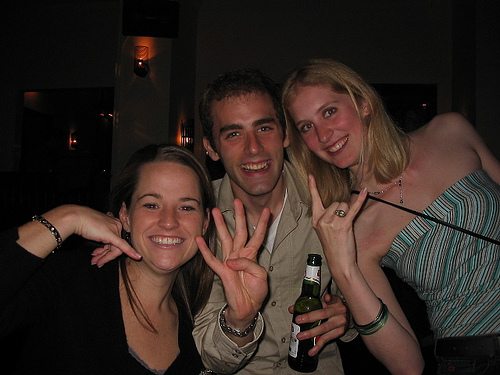
\includegraphics[scale=0.6]{cap4/test_image}
 \caption{Immagine target con tre persone}
 \label{fig:my_label}
 \end{figure}
 
\begin{lstlisting}[h!b]
 >> demo_test
R-CNN startup done
configuring person
Initializing R-CNN model (this might take a little while)
done
Extracting activations from image
Scale = 1.2
Scale = 1
Scale = 0.8
Scale = 0.6
Scale = 0.4
Scale = 0.2
Found 392 activations
Time to detect poselets in image 39.850s
Time to detect bounding boxes in image 40.882s
 \end{lstlisting}
 

 
 \begin{figure}[h]
 \centering
 \subfloat {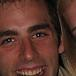
\includegraphics[scale=1]{cap4/test_act1}}
 \hspace{5mm}
 \subfloat {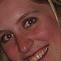
\includegraphics[scale=1]{cap4/test_act2}}
 \hspace{5mm}
 \subfloat {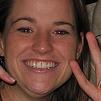
\includegraphics[scale=1]{cap4/test_act3}}

 \subfloat {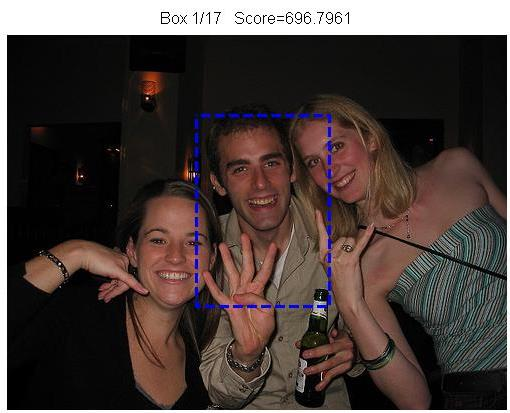
\includegraphics[scale=0.4]{cap4/test_my1}}
 \hspace{5mm}
 \subfloat {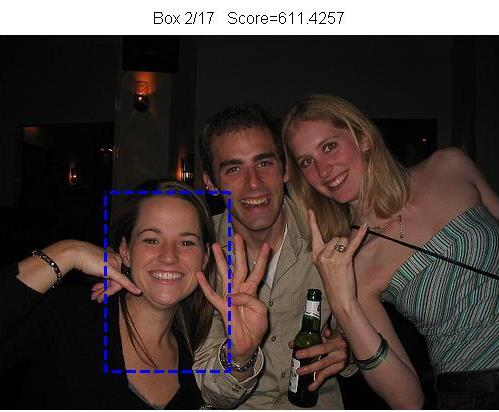
\includegraphics[scale=0.4]{cap4/test_my2}}
 \hspace{5mm}
 \subfloat {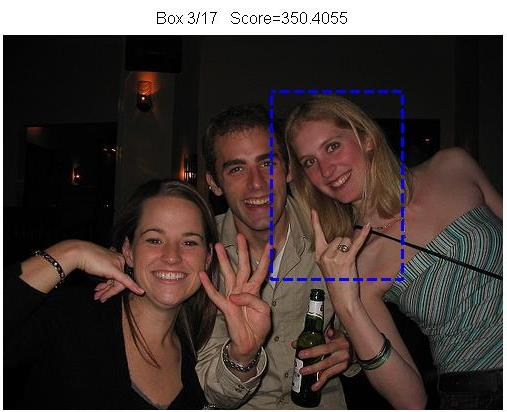
\includegraphics[scale=0.4]{cap4/test_my3}}

 \newline
 \subfloat {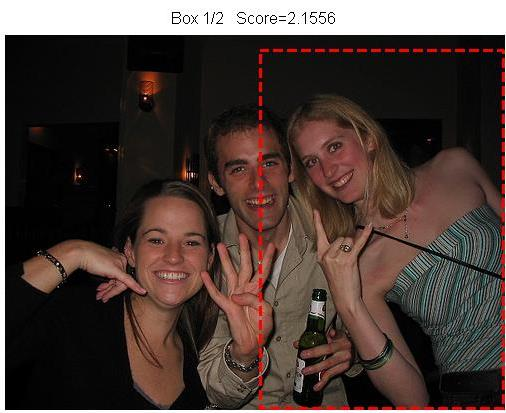
\includegraphics[scale=0.4]{cap4/test_my_rcnn1}}
 \hspace{5mm}
 \subfloat {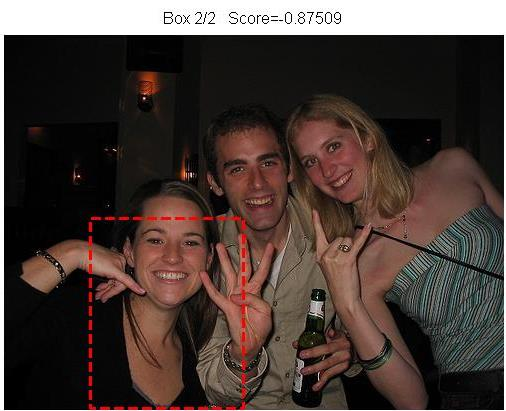
\includegraphics[scale=0.4]{cap4/test_my_rcnn2}}
 
  \subfloat {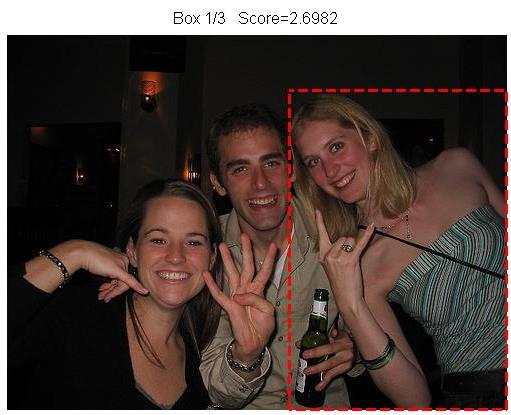
\includegraphics[scale=0.4]{cap4/test_rcnn1}}
 \hspace{5mm}
 \subfloat {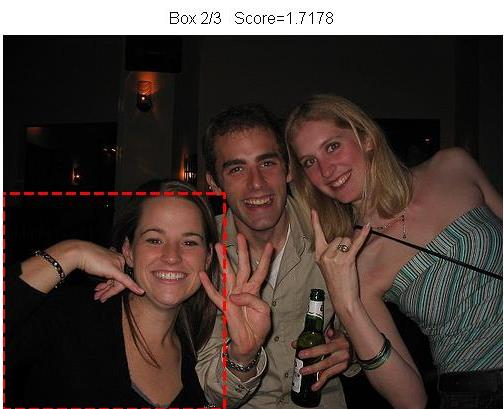
\includegraphics[scale=0.4]{cap4/test_rcnn2}}
 \hspace{5mm}
 \subfloat {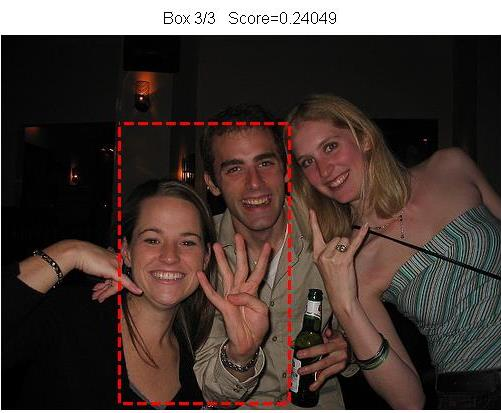
\includegraphics[scale=0.4]{cap4/test_rcnn3}}
\caption{\textbf{Prima riga:} 3 attivazioni-poselet \textbf{Seconda riga:} Primi 3 bounding boxes rilevati dall'approccio. \newline \textbf{Terza riga} Classificazione bounding boxes rilevati da parte di R-CNN\newline
 \textbf{Quarta riga}: Selective Search Candidates + Classificazione mediante R-CNN }
 \end{figure}
 
 Vediamo dalle immagini come R-CNN non riesca a trovare il bounding box che contenga la sola persona al centro. Questo è dovuto a due motivi: il primo è che il classificatore SVM è addestrato per individuare l'intera persona e non parti di esso, il secondo è dovuto all'algoritmo utilizzato per estrapolare le regioni all'interno dell'immagine il quale non sempre funziona a dovere.\\
 
  \begin{figure}[h]
 \centering
 \subfloat {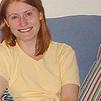
\includegraphics[scale=1]{cap4/test2_act1}}
 \hspace{5mm}
 \subfloat {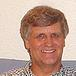
\includegraphics[scale=1]{cap4/test2_act2}}
 \hspace{5mm}
 \subfloat {
\includegraphics[scale=1]{cap4/test2_act3}}

 \newline
 \subfloat {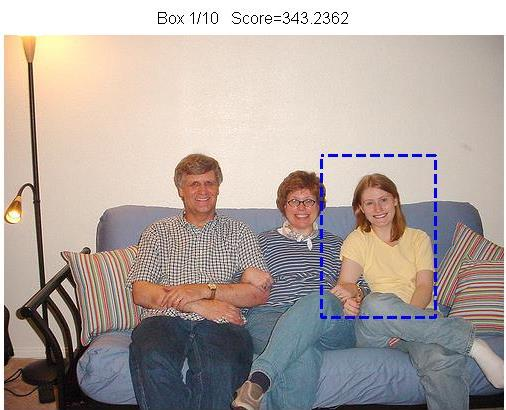
\includegraphics[scale=0.4]{cap4/test2_my1}}
 \hspace{5mm}
 \subfloat {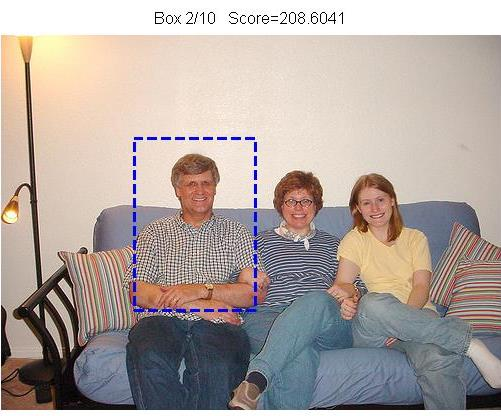
\includegraphics[scale=0.4]{cap4/test2_my2}}
 \hspace{5mm}
 \subfloat {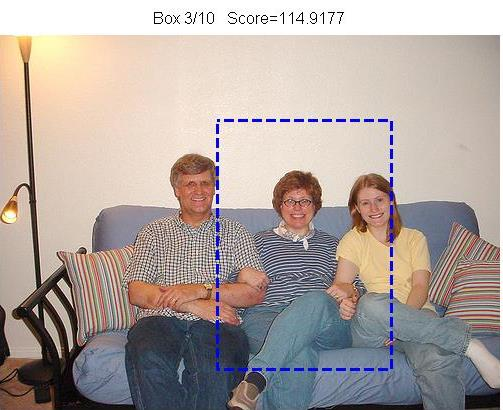
\includegraphics[scale=0.4]{cap4/test2_my3}}

 \newline
 \subfloat {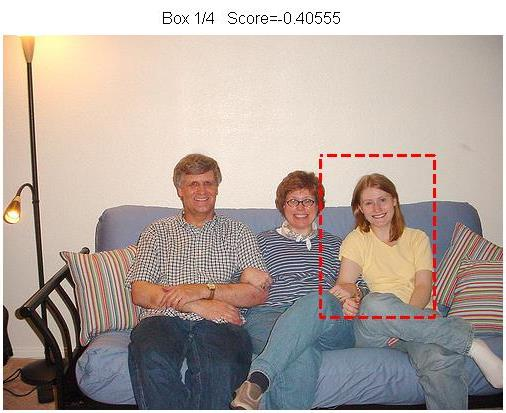
\includegraphics[scale=0.4]{cap4/test2_my_rcnn1}}
 \hspace{5mm}
 \subfloat {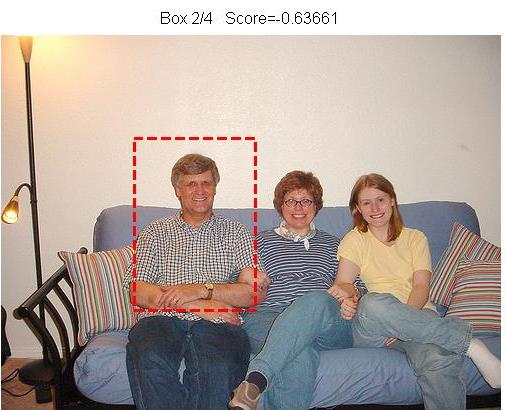
\includegraphics[scale=0.4]{cap4/test2_my_rcnn2}}
 \hspace{5mm}
 \subfloat {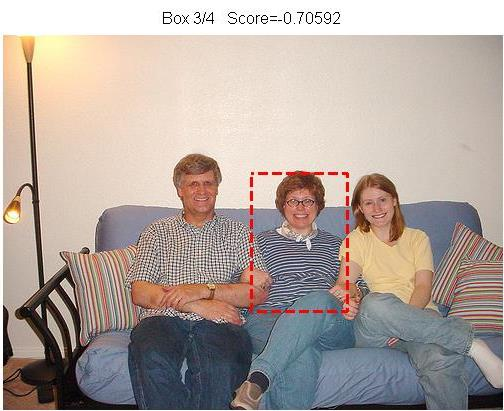
\includegraphics[scale=0.4]{cap4/test2_my_rcnn3}}
 
 \subfloat {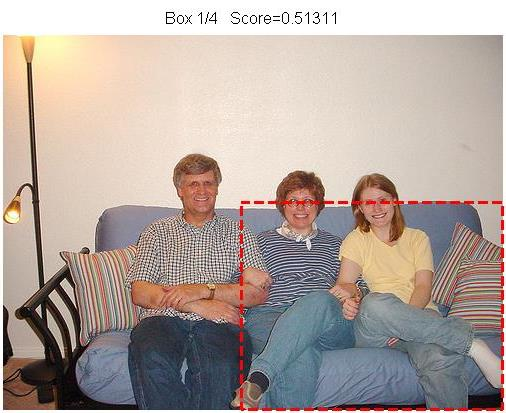
\includegraphics[scale=0.4]{cap4/test2_rcnn1}}
 \hspace{5mm}
 \subfloat {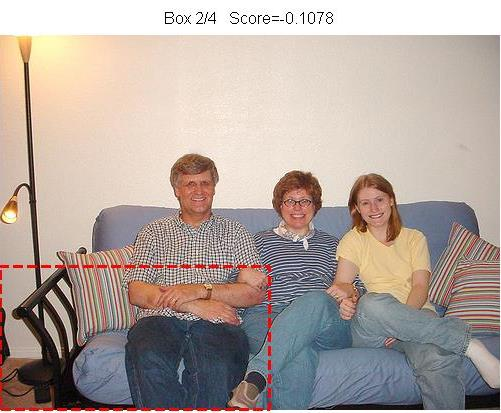
\includegraphics[scale=0.4]{cap4/test2_rcnn2}}
 \hspace{5mm}
 \subfloat {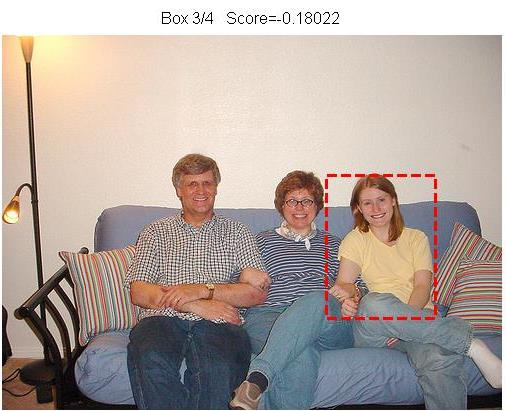
\includegraphics[scale=0.4]{cap4/test2_rcnn3}}
 \caption{\textbf{Prima riga:} 3 attivazioni-poselet \textbf{Seconda riga:} Primi 3 bounding boxes rilevati dall'approccio. \newline \textbf{Terza riga} Classificazione bounding boxes rilevati da parte di R-CNN\newline
 \textbf{Quarta riga}: Selective Search Candidates + Classificazione mediante R-CNN }
 \end{figure}
 
 Nella seconda esecuzione, notiamo che i primi due bounding boxes sono gli stessi sia per l'approccio implementato (score bounding boxes dato dalla somma degli score delle activations all'interno), sia dopo la classificazione di R-CNN. Vediamo come R-CNN col semplice Selective Search Candidates non dia risultati esatti.